\chapter{Implementacija i korisničko sučelje}
		
		
		\section{Korištene tehnologije i alati}
		
			\subsection{Backend tehnologije}
			
			Odabrani programski jezik \textit{backenda} naše web-aplikacije jest \uline{Java}\footnote{\url{https://www.java.com/en/}} u sklopu razvojnog okvira \uline{Spring Boot}\footnote{\url{https://spring.io/}} koji pruža razrađeni model programiranja i konfiguracije te je jedan od najčešće korištenih Java EE okvira za izgradnju aplikacija. Korištene su i pripadne \uline{Spring Data}\footnote{\url{https://spring.io/projects/spring-data}} i \uline{Spring Security}\footnote{\url{https://spring.io/projects/spring-security}} podrške. Za strukturiranje i automatizaciju razvojnog ciklusa projekta korišten je alat \uline{Maven}\footnote{\url{https://maven.apache.org/}}. Odabrani sustav upravljanja relacijskim bazama podataka jest \uline{PostgreSQL}\footnote{\url{https://www.postgresql.org/}}, dok je u razvojnoj i testnoj fazi projekta korišten \textit{in-memory} sustav \uline{H2}\footnote{\url{https://www.h2database.com/}}. Za lakšu navigaciju i testiranje aplikacijskog programskog sučelja  korišten je alat \uline{Swagger UI}\footnote{\url{https://swagger.io/tools/swagger-ui/}}. Za generiranje PDF dokumenata unutar aplikacije,  korištena je knjižica \uline{IText}\footnote{https://itextpdf.com/en}. Korištena razvojna okruženja na \textit{backendu} su \uline{Eclipse IDE}\footnote{\url{https://www.eclipse.org/eclipseide/}} i \uline{IntelliJ IDEA}\footnote{\url{https://www.jetbrains.com/idea/}}.
			
			\subsection{Frontend tehnologije}
			Korisničko sučelje aplikacije temeljeno je na označnom jeziku \uline{HTML5}\footnote{\url{https://html.spec.whatwg.org/}} i stilskom jeziku \uline{CSS}\footnote{\url{https://www.w3.org/Style/CSS/Overview.en.html}} . Modelirano je pomoću razvojnog okvira \uline{React}\footnote{\url{https://reactjs.org/}} u programskom jeziku \uline{JavaScript}. React se koristi za izradu jednostraničnih aplikacija, tj. stranica koje komuniciraju s korisnikom dinamički mijenjajući trenutnu web stranicu umjesto učitavanja cijele nove stranice. Složenije jednostranične aplikacije osim React-a koriste i niz drugih knjižica za nadogradnju komponenti. Za upravljanje knjižicama koristi se \uline{npm}\footnote{\url{https://www.npmjs.com/}}. Neke od mnogih korištenih knjižica u izrađenoj aplikaciji su \uline{Bootstrap}\footnote{\url{https://getbootstrap.com/}}, \uline{Material UI}\footnote{\url{https://material-ui.com/}}, \uline{Semantic UI}\footnote{\url{https://semantic-ui.com/}} i \uline{Redux}\footnote{https://redux.js.org/}. Korištena razvojna okolina na \textit{frontendu} jest \uline{Visual Studio Code}\footnote{\url{https://code.visualstudio.com/}}.
			
			 \subsection{Puštanje u pogon}
            Cijeli sustav uspostavljen je i pušten u pogon na platformi \uline{Heroku}\footnote{\url{https://www.heroku.com/}}, servisu temeljenom na oblaku.
            
			\subsection{Dokumentacija}
			Za dokumentaciju programskog riješenja korišten je \uline{Astah}\footnote{https://astah.net/}, alat za modeliranje UML dijagramima. Za vizualizaciju i modeliranje baze podataka korišten je alat \uline{Erdplus}\footnote{https://erdplus.com/}.
			
			\subsection{Timska komunikacija}
			Za svrhe komunikacije unutar tima korištene su sljedeće platforme: 
			\begin{itemize}
			    \itemsep-0.5em
			    \item  \uline{Trello}\footnote{\url{https://trello.com/en}} - organizacijska platforma temeljena na kanban metodi
			    \item \uline{Discord}\footnote{\url{https://discord.com/}} - VoIP platforma za brzu komunikaciju
			    \item \uline{WhatsApp}\footnote{\url{https://www.whatsapp.com/}} - aplikacija za razmjenu poruka
			    \item \uline{Microsoft Teams}\footnote{\url{https://www.microsoft.com/en-us/microsoft-365/microsoft-teams/group-chat-software}} -  platforma za video konferencije
			\end{itemize}
			\medskip
			\noindent Za distribuirano upravljanje kodom i verzioniranje korišten je sustav \uline{Git}\footnote{\url{https://git-scm.com/}} s udaljenim repozitorijem posluženim na \uline{GitLab}\footnote{\url{https://about.gitlab.com/}} platformi.
	        \eject 
		
	
		\section{Ispitivanje programskog rješenja}
			
			\subsection{Ispitivanje komponenti}
			
			Uspješna rezervacija je temeljna funkcionalnost ove aplikacije. JUnit testovima ispitani su rubni i redovni slučajevi te oni koji izazivaju pogreške. Priložen je kod kojim su u bazu dodani entiteti potrebni za ispitivanje funkcionalnosti rezervacije te kod Junit testova. 
			
			\begin{figure}[H]
				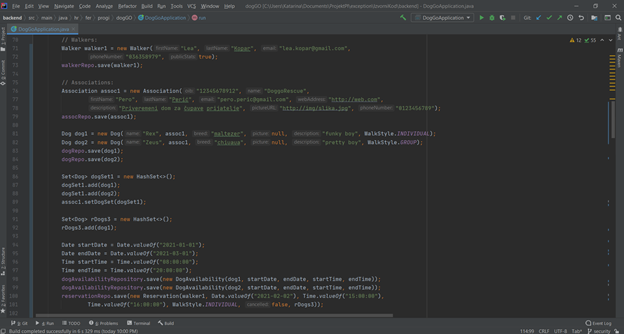
\includegraphics[scale=1]{slike/ispitivanje-sustava-1.png} 
				\centering
				\caption{Prikaz inicijalizacije testnih podataka}
				\label{fig:testiranje}
			\end{figure}
			
			\noindent \textbf{Ispitni slučaj 1: Pokušaj rezervacije gdje je sat početka vremenski nakon sata završetka šetnje}
			
			Nije moguće napraviti rezervaciju na isti dan, a da je pritom vrijeme početka šetnje veće od vremena završetka šetnje. Sljedećim testom izazivamo iznimku RequestDeniedException s odgovarajućom porukom
			
			\begin{figure}[H]
				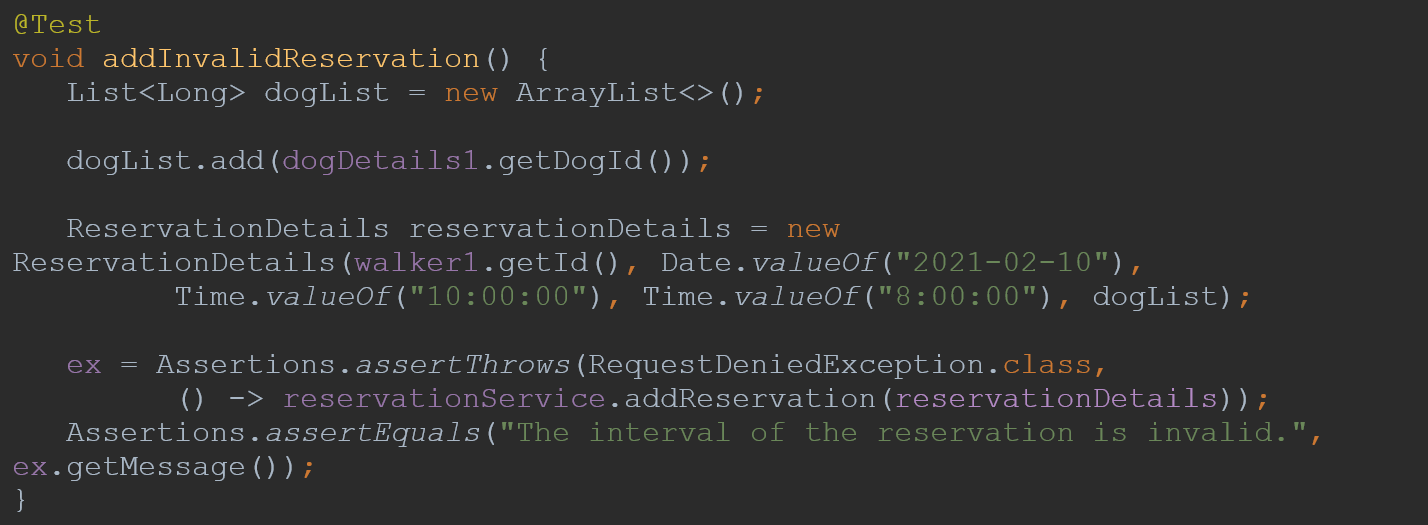
\includegraphics[scale=0.6]{slike/junit-1.PNG}
				\centering
				\caption{Prikaz 1. Junit testa}
				\label{fig:testiranje}
			\end{figure}
			
			\noindent \textbf{Ispitni slučaj 2: Pokušaj rezervacije gdje je pas za grupnu šetnju jedini u rezervaciji}
			
			Psi koji su namijenjeni grupnoj šetnji ne mogu biti jedini u rezervaciji, stoga sljedećim testom želimo napraviti rezervaciju s listom pasa koja ima samo jednog psa, a koji mora biti u grupi s još minimalno jednim psom da bi rezervacija bila uspješna. Pokušaj rezervacije završava iznimkom RequestDeniedException s odgovarajućom porukom.
			
			\begin{figure}[H]
				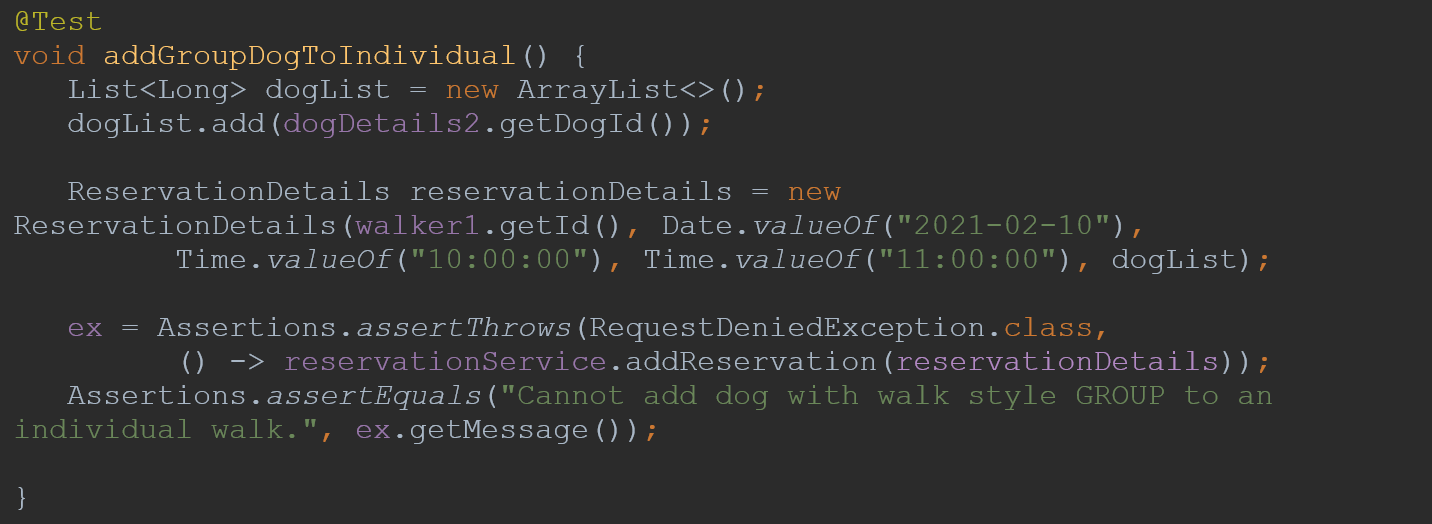
\includegraphics[scale=0.6]{slike/junit-2.PNG}
				\centering
				\caption{Prikaz 2. Junit testa}
				\label{fig:testiranje}
			\end{figure}
			
			\noindent \textbf{Ispitni slučaj 3: Pokušaj rezervacije gdje je pas za individualnu šetnju dodan u grupnu šetnju}
			
			Psi koji su namijenjeni individualnoj šetnji ne mogu biti stavljeni u grupnu šetnju, pa pokušaj rezervacije gdje je takav pas stavljen u grupu s drugima izaziva RequestDeniedException iznimku s odgovarajućom porukom.
			
			\begin{figure}[H]
				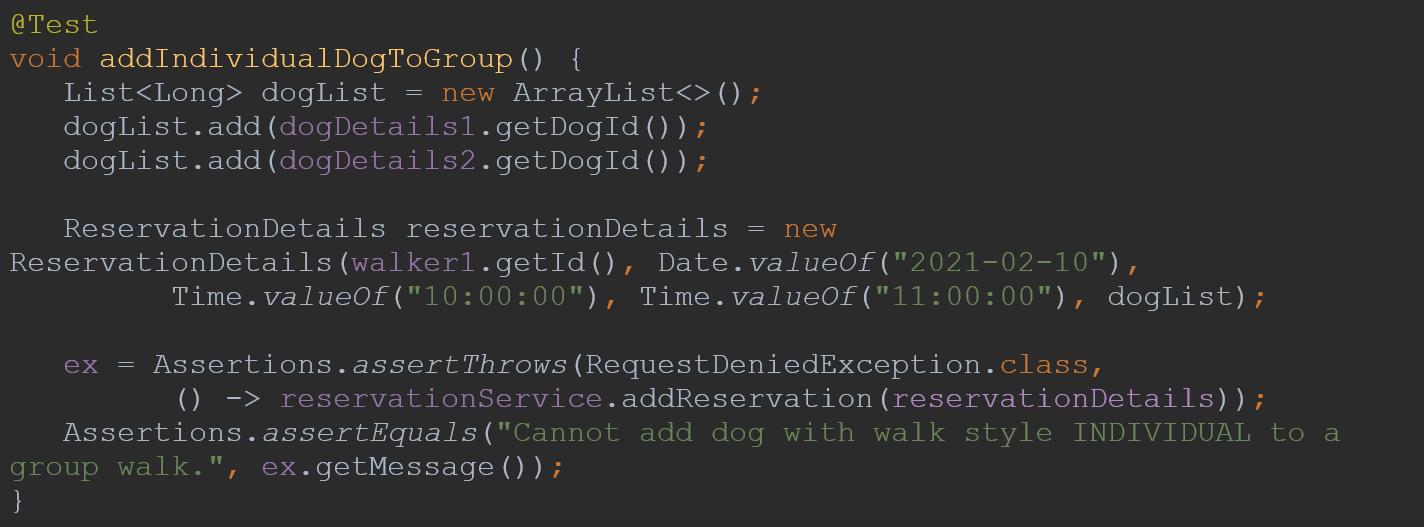
\includegraphics[scale=0.6]{slike/junit-3.PNG}
				\centering
				\caption{Prikaz 3. Junit testa}
				\label{fig:testiranje}
			\end{figure}
			
			\noindent \textbf{Ispitni slučaj 4: Pokušaj rezervacije kada je pas nedostupan}
			
			Ako se pokuša napraviti rezervacija u terminu kada pas nije dostupan, potrebno je izazvati iznimku RequestDeniedException s odgovarajućom porukom.
			
			\begin{figure}[H]
				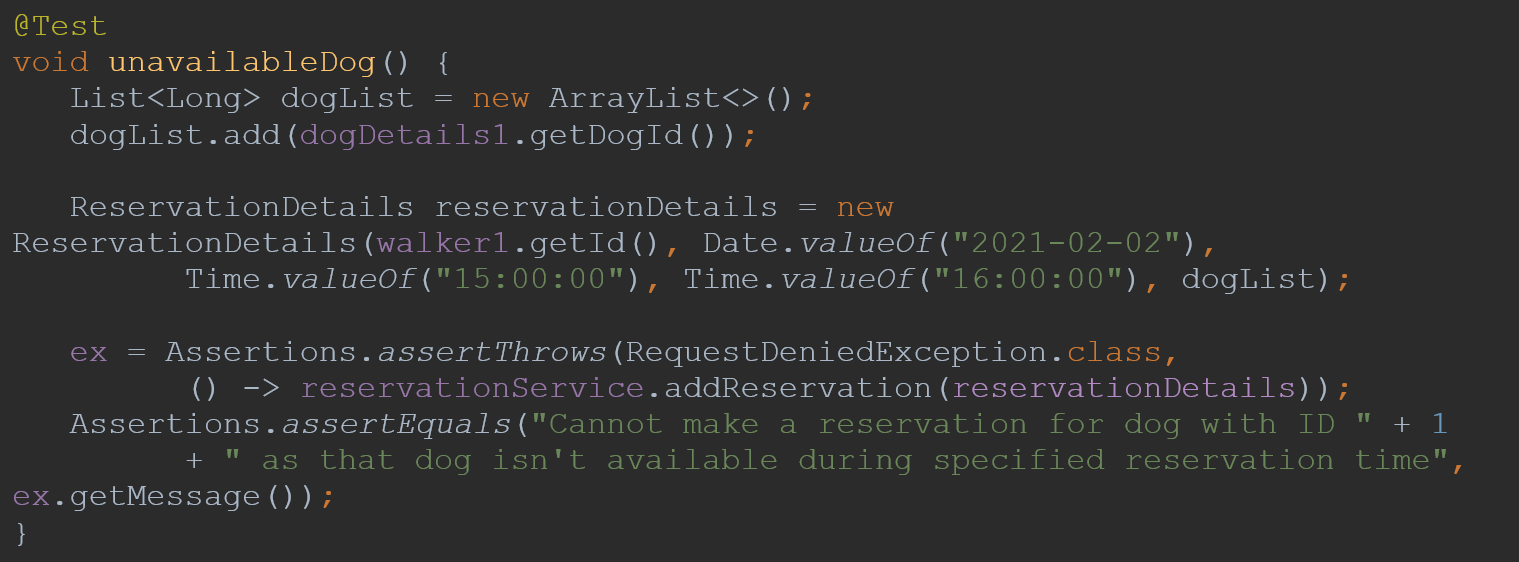
\includegraphics[scale=0.6]{slike/junit-4.PNG}
				\centering
				\caption{Prikaz 4. Junit testa}
				\label{fig:testiranje}
			\end{figure}
			
			\noindent \textbf{Ispitni slučaj 5: Pokušaj rezervacije kada je šetač nedostupan}
			
    		Ako šetač pokuša napraviti rezervaciju u terminu u kojem je već prije napravio rezervaciju također se izaziva RequestDeniedException s odgovarajućom porukom. 
			
			\begin{figure}[H]
				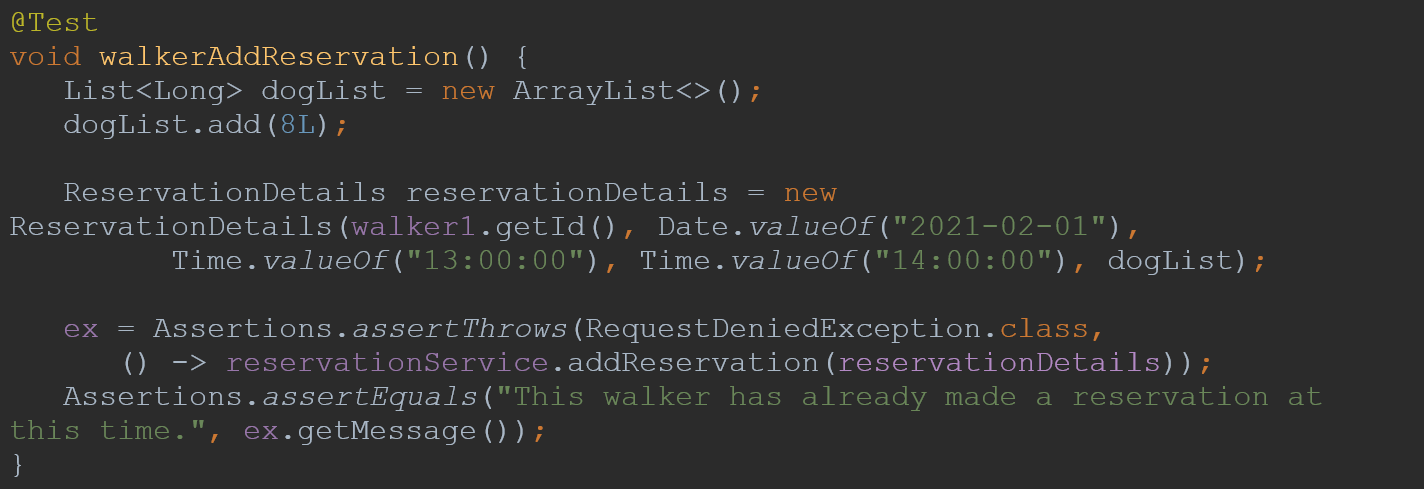
\includegraphics[scale=0.6]{slike/junit-5.PNG}
				\centering
				\caption{Prikaz 5. Junit testa}
				\label{fig:testiranje}
			\end{figure}
			
			\noindent \textbf{Ispitni slučaj 6: Pokušaj rezervacije kada je šetač nedostupan}
			
    		Najbitnije je ispitati je li rezervacija koja ispunjava sve uvjete uspješno napravljena. Sljedećim testom provjeravamo jednakost hardkodiranih detalja rezervacije i detalja metode kojom vraćaju detalji uspješne rezervacije.
			
			\begin{figure}[H]
				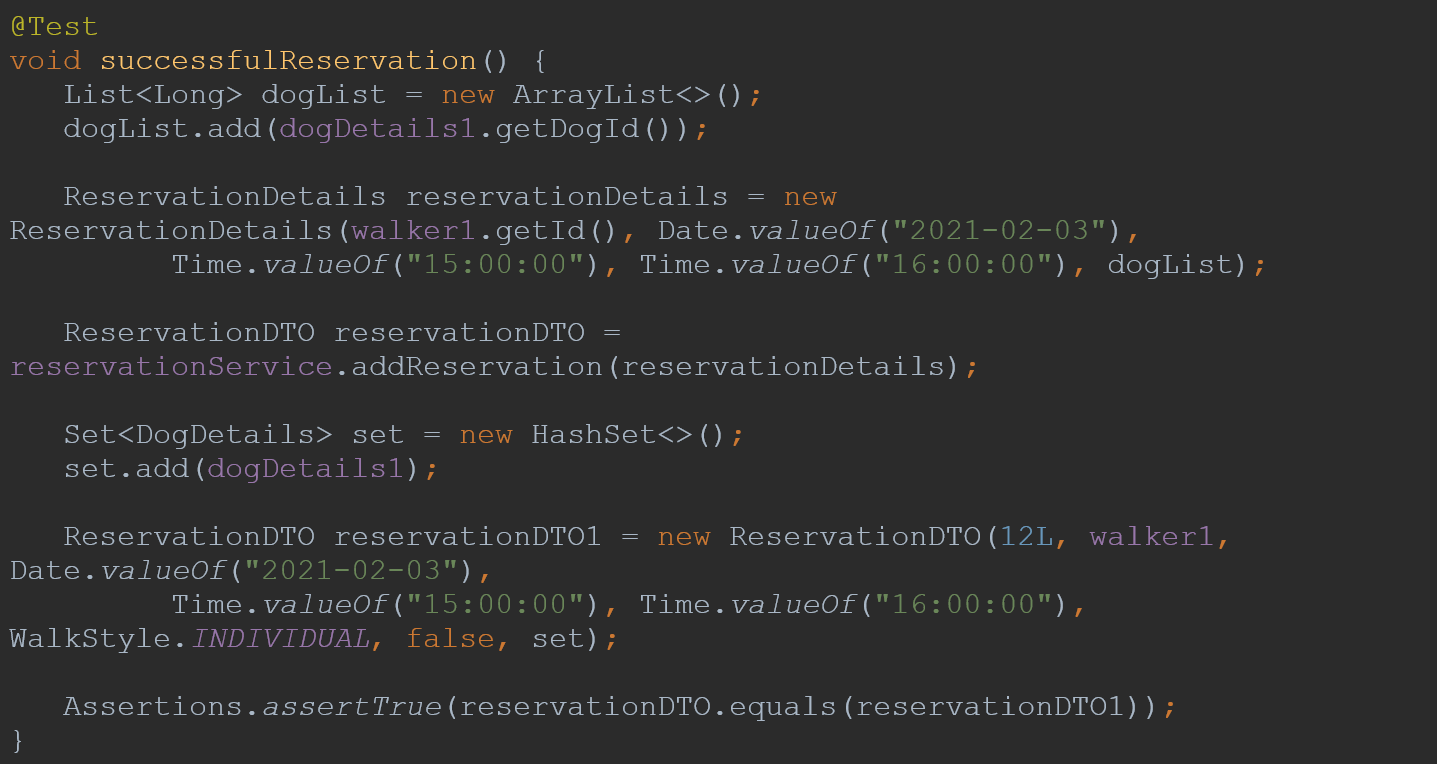
\includegraphics[scale=0.6]{slike/junit-6.PNG}
				\centering
				\caption{Prikaz 6. Junit testa}
				\label{fig:testiranje}
			\end{figure}
			
			\noindent \textbf{Rezultati testiranja}
			
			Svi navedeni Junit testovi su se uspješno proveli.
			
			\begin{figure}[H]
				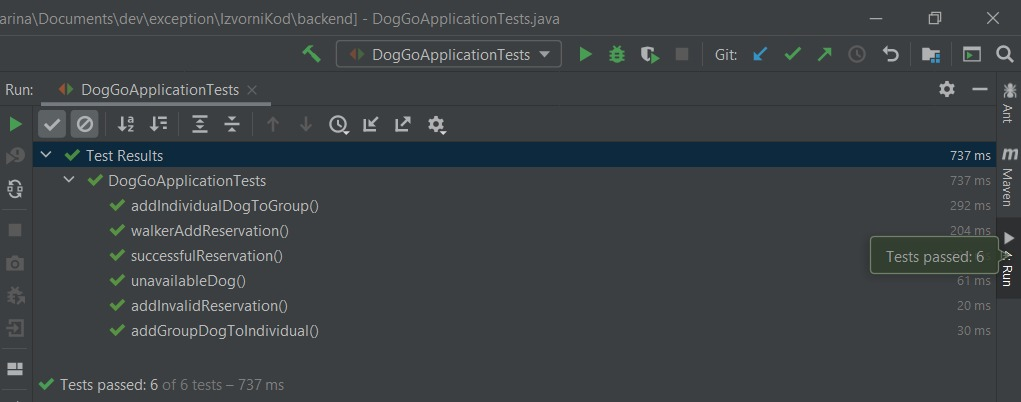
\includegraphics[scale=0.4]{slike/tests-passed.JPEG}
				\centering
				\caption{Prikaz rezultata testova}
				\label{fig:testiranje}
			\end{figure}
			
			\subsection{Ispitivanje sustava}
			
			\noindent \textbf{Ispitni slučaj 1: Rezervacija šetnje}
			
			\noindent \textbf{Ulaz:}
			\begin{packed_enum}
				
				\item Otvaranje početne stranice u web pregledniku.
				\item Otvaranje stranice popisa udruge.
				\item Odabir udruge i pritisak kursorom na gumb REZERVIRAJ.
				\item Odabir datuma i vremenskog intervala šetnje.
				\item Pritisak kursorom na gumb Rezerviraj.
				
			\end{packed_enum}
			\textbf{Očekivani rezultat:}
			\begin{packed_enum}
				
				\item Prikaz naslovne stranice.
				\item Prikaz popisa udruge.
				\item Prikaz profila udruge i popis pasa.
				\item Prikaz forme za rezervaciju i prikaz odabranog datuma i vremenskih intervala šetnje.
				\item Prikaz poruke uspješne rezervacije i profila udruge.
				
			\end{packed_enum}
			\textbf{Rezultat:} Očekivani rezultat [4.] nije zadovoljen jer je isteklo implicitno vrijeme čekanja. Zbog toga se očekivani rezultat [5.] nije odradio. \textcolor{red}{Aplikacija nije prošla test.}
			
			\begin{figure}[H]
				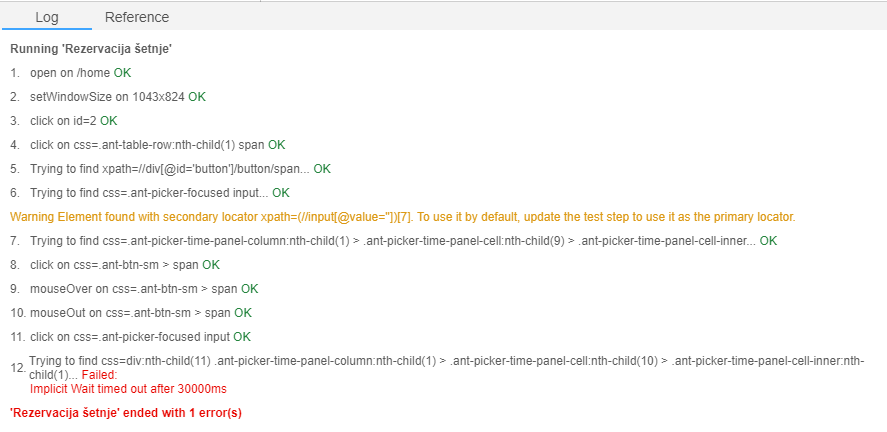
\includegraphics[scale=0.6]{slike/rezervacijaSetnje.PNG} 
				\centering
				\caption{Prikaz rezultata 1. ispitnog slučaja u Selenium-u}
				\label{fig:sustav-prvi-slucaj}
			\end{figure}
		
			\noindent \textbf{Ispitni slučaj 2: Otkazivanje šetnje od strane udruge}
			
			\noindent \textbf{Ulaz:}
			\begin{packed_enum}
				
				\item Otvaranje početne stranice u web pregledniku.
				\item Otvaranje profila udruge.
				\item Odabir popisa rezervacija udruge.
				\item Pritisak kursorom na gumb OTKAŽI.
				
			\end{packed_enum}
			\textbf{Očekivani rezultat:}
			\begin{packed_enum}
				
				\item Prikaz naslovne stranice.
				\item Prikaz profila udruge i popis pasa.
				\item Prikaz popisa rezervacija na profilu udruge.
				\item Prikaz profila udruge i popis pasa.
				
			\end{packed_enum}
			\textbf{Rezultat:} \textcolor{red}{Aplikacija je prošla test.}
			
			\begin{figure}[H]
				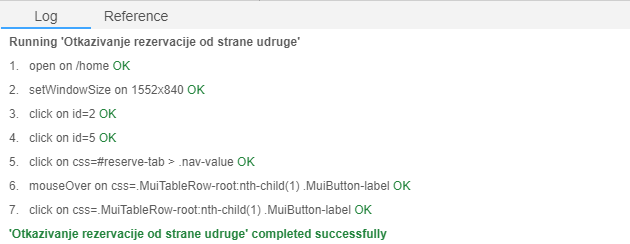
\includegraphics[scale=0.7]{slike/otkazivanjeRezervacijeOdStraneUdruge.PNG} 
				\centering
				\caption{Prikaz rezultata 2. ispitnog slučaja u Selenium-u}
				\label{fig:sustav-drugi-slucaj}
			\end{figure}
		
			\noindent \textbf{Ispitni slučaj 3: Otkazivanje šetnje od strane admina}
			
			\noindent \textbf{Ulaz:}
			\begin{packed_enum}
				
				\item Otvaranje početne stranice u web pregledniku.
				\item Otvaranje admin profila.
				\item Pomicanje ekrana do prikaza popisa rezervacija.
				\item Pritisak kursorom na gumb OTKAŽI.
				
			\end{packed_enum}
			\textbf{Očekivani rezultat:}
			\begin{packed_enum}
				
				\item Prikaz naslovne stranice.
				\item Prikaz admin profila.
				\item Prikaz popisa rezervacija na admin profilu.
				\item Prikaz ažuriranog popisa rezervacija na admin profilu.
				
			\end{packed_enum}
			\textbf{Rezultat:} \textcolor{red}{Aplikacija je prošla test.}
			
			\begin{figure}[H]
				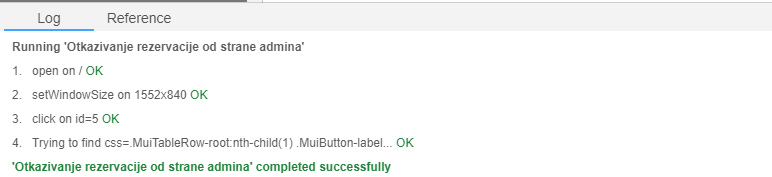
\includegraphics[scale=0.7]{slike/otkazivanjeRezervacijeOdStraneAdmina.PNG} 
				\centering
				\caption{Prikaz rezultata 3. ispitnog slučaja u Selenium-u}
				\label{fig:sustav-treci-slucaj}
			\end{figure}
			\eject 
		
		
		\section{Dijagram razmještaja}
			
			 Dijagram razmještaja opisuje topologiju sustava i usredotočen je na odnos sklopovskih i programskih dijelova. 
			 Arhitektura sustava DogGO aplikacije je ”klijent – poslužitelj” gdje web poslužitelj i poslužitelj baze podataka se nalaze na poslužiteljskom računalu a klijenti koriste web preglednik kako bi pristupili web aplikaciji. Komunikacija između računala korisnika i poslužitelja odvija se preko HTTP veze.
			 
			 \begin{figure}[H]
				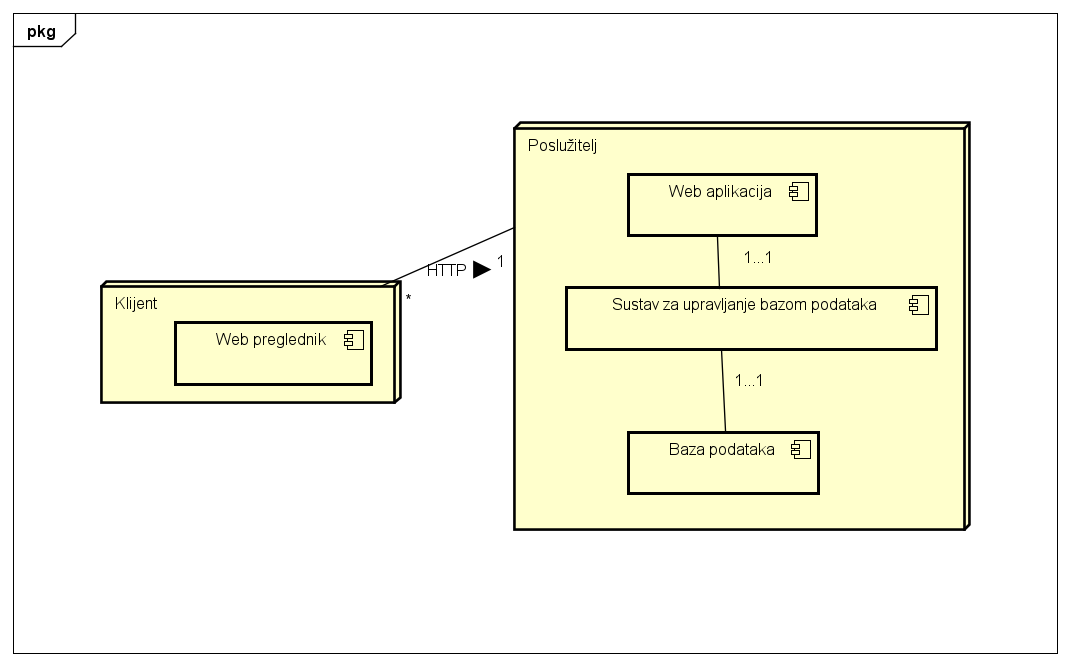
\includegraphics[scale=0.6]{dijagrami/deploy.png} 
				\centering
				\caption{Dijagram razmještaja}
				\label{fig:dijagram-razmjestaja}
			\end{figure}
			
			\eject 
		
		\section{Upute za puštanje u pogon}
			
			Puštanje aplikacije u pogon možemo podijeliti na 3 glavna koraka
			         \begin{packed_item}
                            \item[$\bullet$] pokretanje Postgres baze
                            \item[$\bullet$] pokretanje backenda (Spring Boot)
                            \item[$\bullet$] pokretanje frontenda (npm, React)
                    \end{packed_item}
                    
                \subsection{Pokretanje baze}
                
                Za pokretanje baze prvo je potrebno skinuti Postgres bazu. Preuzmemo installer sa \textit{https://www.postgresql.org/download/} (verzija 13), te slijedimo upute za instalaciju. Zatim preuzimamo i instaliramo PgAdmin (\textit{https://www.pgadmin.org/download/}), koji nam olakšava upravljanje bazom i pregled podataka. \newline
                
                \noindent Nakon instalacije navedenih komponenti, moramo još kreirati bazu, odnosno korisničko ime koje ćemo koristiti za spajanje na bazu.\newline
                
                \noindent 1) Otvorimo pgAdmin. Prilikom prvog pokretanja, aplikacija nas traži upisivanje glavne lozinke, koji smislimo i upišemo. Zatim klikom na Login/Group Roles -> Create otvaramo izbornik za stvaranje novog korisnika.
                
                    \begin{figure}[H]
        				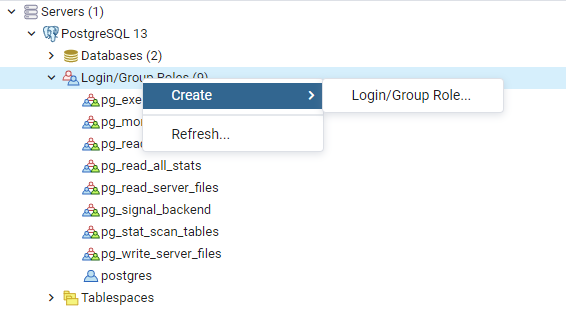
\includegraphics[scale=0.6]{slike/deploy_kreiranje_usera1.PNG} 
        				\centering
        				\caption{Kreiranje usera}
        				\label{fig:sustav-prvi-slucaj}
        			\end{figure}
        			
        		U odgovarajuća polja upišemo željeno korisničko ime i password (u primjeru korišten exampleUser/password123)
                
                    \begin{figure}[H]
        				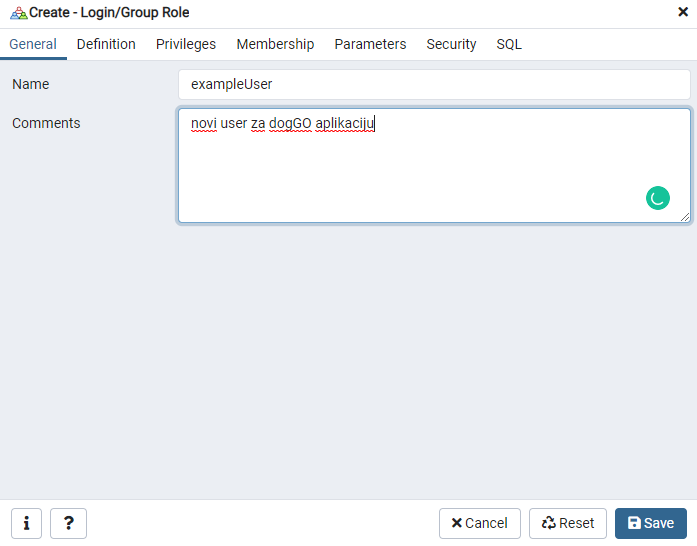
\includegraphics[scale=0.6]{slike/deploy_kreiranje_usera2.PNG} 
        				\centering
        				\caption{Kreiranje usera - upis korisničkog imena}
        				\label{fig:sustav-prvi-slucaj}
        			\end{figure}
        			
        			 \begin{figure}[H]
        				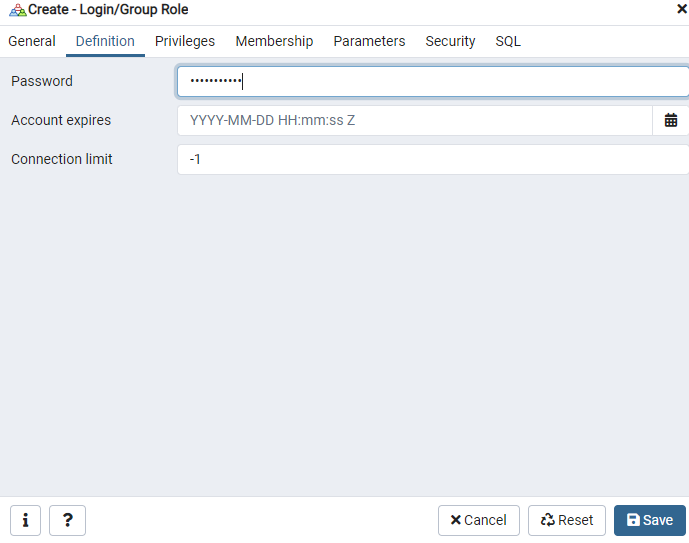
\includegraphics[scale=0.6]{slike/deploy_kreiranje_usera3.PNG} 
        				\centering
        				\caption{Kreiranje usera 3 - upis lozinke}
        				\label{fig:sustav-prvi-slucaj}
        			\end{figure}
                
                Nakon što smo stvorili korisnika, možemo stvoriti i novu bazu.
                
                    \begin{figure}[H]
        				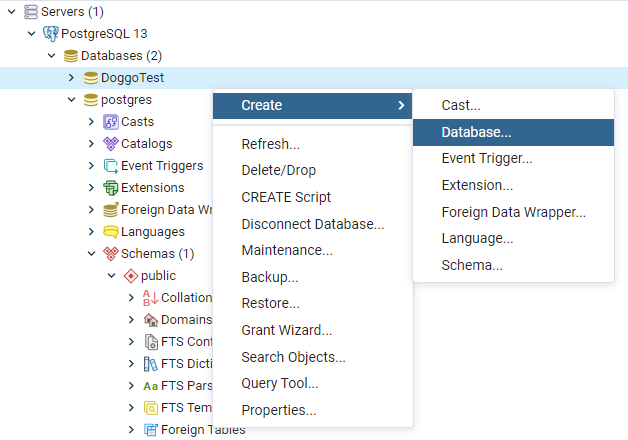
\includegraphics[scale=0.6]{slike/deploy_kreiranje_baze1.PNG} 
        				\centering
        				\caption{Izbornik za stvaranje baze}
        				\label{fig:sustav-prvi-slucaj}
        			\end{figure}
        			
        			Jedino što je potrebno upisati je ime baze (u primjeru DoggoExample), te vlasnika baze - novostvoreni korisnik exampleUser.
        			
        			 \begin{figure}[H]
        				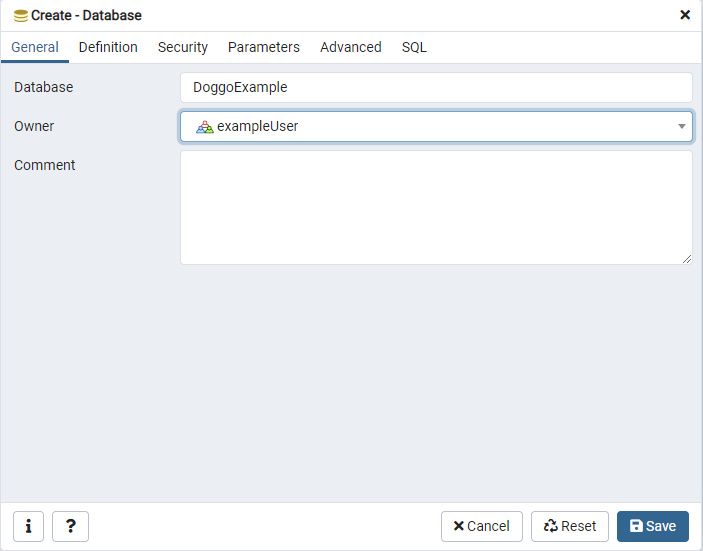
\includegraphics[scale=0.6]{slike/deploy_kreiranje_baze2.PNG} 
        				\centering
        				\caption{Izbornik za stvaranje baze - upis imena i vlasnika}
        				\label{fig:sustav-prvi-slucaj}
        			\end{figure}
        			
        			
                
                \subsection{Pokretanje backenda}
                
                Za ispravno pokretanje backenda, prvo moramo instalirati sljedeće aplikacije
			         \begin{packed_item}
                            \item[$\bullet$] alat za upravljanje kodom Maven (najnovija trenutačna verzija). Ukoliko se backend pokreće iz naredbenog retka sa naredbom mvnw, instalacija nije potrebna (tj. mvnw je maven wrapper, program koji sam preuzima i privremeno instalira potrebnu verziju Mavena)
                            \begin{packed_item}
                                \item[$\bullet$] za instalaciju slijedimo upute na \textit{https://maven.apache.org/install.html}
                            \end{packed_item}
                            \item[$\bullet$] Java verzije 15 ili novija
                            \begin{packed_item}
                                \item[$\bullet$] za instalaciju slijedimo upute na \textit{https://docs.oracle.com/en/java/javase/15/install/overview-jdk-installation.html}
                            \end{packed_item}
                            \item[$\bullet$] (opcionalno) neki IDE (IntelliJ/Eclipse)
                    \end{packed_item}
                    
                    \noindent Nakon preuzimanja svih potrebnih aplikacija, prvo moramo podesiti spajanje na našu novostvorenu bazu. U nekom uređivaču teksta ili IDE-u otvorimo datoteku IzvorniKod/backend/src/main/java/resources/application.properties, te tamo unesemo sljedeće podatke:
                    
                    \begin{figure}[H]
        				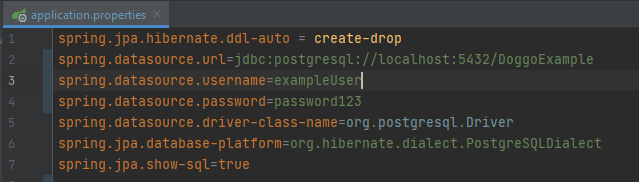
\includegraphics[scale=0.6]{slike/deploy_applicationproperties.PNG} 
        				\centering
        				\caption{application.properties}
        				\label{fig:sustav-prvi-slucaj}
        			\end{figure}
                    
                    U ovom trenutku imamo sve spremno za pokretanje backenda, što možemo učiniti na 2 načina:\newline \\
                    
                    \noindent a) Korištenjem naredbenog retka (command line)
                    Za pokretanje iz naredbenog retka korištenjem Windows powershella/Linux terminala ili slično pozicioniramo se u direktorij IzvorniKod/backend/
                    te tamo pokrenemo naredbu \textbf{mvn clean install}. Nakon dovršenja ove naredbe, iz istog direktorija pokrenemo i \textbf{mvn spring-boot:run}. Aplikacija se pokrenula na URL-u http://localhost:8080.\newline

                    \noindent b) Korištenjem IDE-a (IntelliJ)
                    Za pokretanje aplikacije iz IDE-a, prvo moramo otvoriti naš projekt u IntelliJ-u. 
                    Klikom na File/Open otvara nam se izbornik u kojem pronađemo naš projekt te u njemu odaberemo folder backend.
                    
                    \begin{figure}[H]
        				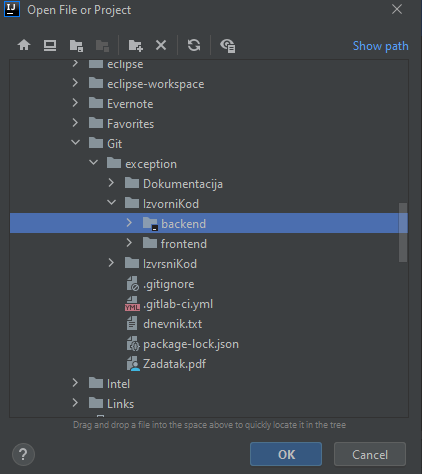
\includegraphics[scale=0.6]{slike/deploy_ideizbornik.PNG} 
        				\centering
        				\caption{Otvaranje projekta u IntelliJ-u}
        				\label{fig:sustav-prvi-slucaj}
        			\end{figure}
        			
        			Nakon otvaranja projekta, u gornjem desnog uglu pronađemo zelenu ikonicu u obliku trokuta, te ju kliknemo. Klikom na nju, aplikacija se pokreće na URL-u http://localhost:8080.
        			
        			 \begin{figure}[H]
        				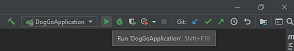
\includegraphics[scale=1]{slike/deploy_runappide.PNG} 
        				\centering
        				\caption{Pokretanje aplikacije iz IntelliJ-a}
        				\label{fig:sustav-prvi-slucaj}
        			\end{figure}
        			
                \subsection{Pokretanje frontenda}
                
                Za pokretanje iz naredbenog retka potrebno se pozicionirati u direktorij IzvorniKod/frontend/app/src i u njemu izvesti sljedeće naredbe:

                \textbf{npm install}
                
                \noindent Naredba instalira sve node module potrebne za pokretanje aplikacije.\newline
                
                \textbf{npm start}
                
                \noindent Pokreće aplikaciju na http://localhost:3000.
                Stranica se ponovno učitava svakom spremljenom promjenom u kodu.

			
			
			\eject 